\chapter{Ideal Gases}

\subsection{Gas molecules}


\subsection{Motion of gas particles} \label{s-gas-intro}

\begin{marginfigure}
	\centering
	
	\vspace*{-20pt}
	
	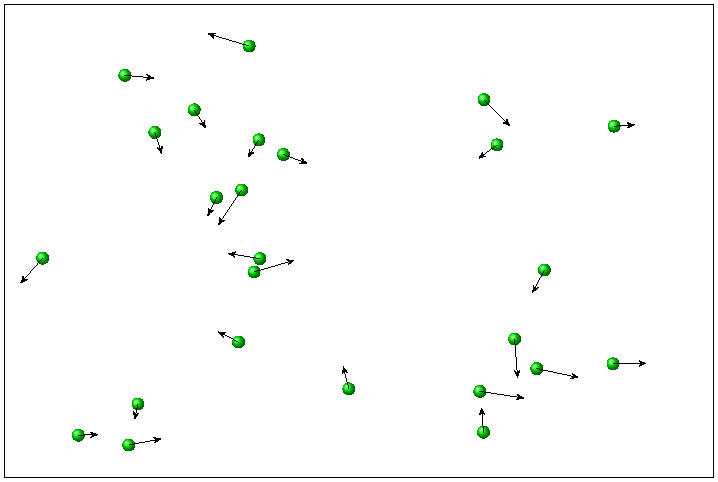
\includegraphics[width=6cm]{gas-random-motion}
		
	\caption{The motion of gas molecules in a container}
	
\end{marginfigure}

Our core assumption for ideal gasses is that a gas consists of a large number of molecules. These gas molecules move \emph{randomly} at high speeds and the  randomness results from \emph{collisions} of fast-moving molecules in the gas.

We assume that for an individual molecule, its velocity changes constantly as it collides with other molecules so at any instant, there is a range of molecule velocities.  

There is some strong evidence of random motion often referred to as \keypoint{Brownian motion}\footnote{We attribute the discovery of this random motion to the botanist Robert brown but there are many earlier descriptions from the early greeks - or this remarkable description of dust molecules from the roman Lucretius: \begin{quote}
    
``Observe what happens when sunbeams are admitted into a building and shed light on its shadowy places. You will see a multitude of tiny particles mingling in a multitude of ways... their dancing is an actual indication of underlying movements of matter that are hidden from our sight... It originates with the atoms which move of themselves [i.e., spontaneously]. Then those small compound bodies that are least removed from the impetus of the atoms are set in motion by the impact of their invisible blows and in turn cannon against slightly larger bodies. So the movement mounts up from the atoms and gradually emerges to the level of our senses so that those bodies are in motion that we see in sunbeams, moved by blows that remain invisible.''\end{quote}}\index{Brownian motion}. If you observe a dust mote or smoke particles in the air, you'll see that they undergo jerky random motion due to collisions with the randomly moving gas molecules. 

We know also from these observations that the speed of gas molecules depend on temperature, molecules move faster at higher temperature\footnote{We will prove this statement later in this chapter.}.


\subsection{Number of molecules}

In any tangible sample of gas, there are a huge number of molecules. We introduce the mole as a universally accepted \keypoint{amount of a substance}\index{amount of substance} to measure the size of a collection of particles.

\cmt unit of amount of substance: $[n] = \text{mol}$

\begin{ilight}
	One \keypoint{mole} is defined as the amount carbon-12 atoms in a sample of 12 grams. 1 mole of any substance contains 6.02$\times$10$^{23}$ particles
\end{ilight}

This number is called \keypoint{Avogadro constant}\index{Avogadro constant}: $N_A = 6.02\times10^{23} \text{ mol}^{-1}$ \footnote{In 2018, IUPAC suggested a new definition of the mole, which is defined to contain exactly 6.02$\times$10$^{23}$ particles. This new definition fixed numerical value of the Avogadro constant, and emphasized that the quantity `amount of substance' is concerned with counting number of particles rather than measuring the mass of a sample.}

With the constant being just a number, it's easy to convert between number of molecules and amount of substance: $\tcbhighmath{N=nN_A}$

One of the useful shortcuts that the mole grant us is the notion of molar mass $M$

\begin{ilight}
	\keypoint{Molar mass}\index{molar mass} of a substance is defined as the mass of a given sample divided by the amount of substance: $M=\frac{m}{n}$
\end{ilight}

\begin{compactitem}
	\item[--] $\text{amount of substance} = \frac{\text{mass of sample}}{\text{molar mass}}$, or $n = \frac{m}{M}$
	
	\eqyskip
	
	\item[--] $\text{mass of single molecule} = \frac{\text{molar mass}}{\text{Avogadro constant}}$, or $m_0 = \frac{M}{N_A}$
\end{compactitem}

\example{Find the number of molecules in 160 grams of argon-40 gas.}

\begin{soln} Amount of gas: $n=\frac{m}{M} = \frac{160 \text{ g}}{40 \text{ g mol}^{-1}} = 4.0 \text{ mol}$

number of gas molecules: $N = n N_A = 4.0 \text{ mol} \times 6.02\times10^{23} \text{ mol}^{-1} \approx 2.41 \times 10^{24}$ \end{soln}

\question{Find the mass of a sample of uranium-235 that contains $6.0\times10^{20}$ atoms.}
	




\subsection{Pressure (qualitative view)}

When gas molecules collide with walls of container and rebound, they change their momentum. By Newton's second law there must be a force on them from the wall of the container. By Newton's third law, gas molecules must exert a reaction force on container. The contributions from many molecules give rise to a constant pressure.

\example{If a gas is heated with its volume fixed, how does the pressure change?}

\begin{soln}At higher temperature, gas molecules move faster

they will collide \emph{harder} and produce a greater force upon each collision

they will also collide more \emph{frequently} with the container

so pressure of the gas will increase \end{soln}

\question{If you pump gas into a bicycle tyre, state and explain how the pressure changes.}

\question{A fixed amount of gas is allowed to expand at constant temperature, state and explain how the pressure changes.}





\subsection{Empirical laws}

In 1643, the Italian physicist and mathematician, Evangelista Torricelli, who for a few months had acted as Galileo's secretary, conducted a celebrated experiment in Florence. He demonstrated that a column of mercury in an inverted tube can be supported by the pressure of air outside of the tube, with the creation of a small section of vacuum above the mercury. This experiment essentially paved the way towards the invention of the barometer, as well as drawing the attention of Robert Boyle, then a "skeptical" scientist working in England. Boyle was inspired by Torricelli's experiment to investigate how the elasticity of air responds to varying pressure, and he did this through a series of experiments performed by his assistant \emph{Robert Hooke}\footnote{Yes, that Hooke, of Hooke's law.}

\subsection*{Boyle's law}\index{Boyle's law}

Boyle's law was discovered by \emph{Robert Boyle} in 1662, based on experimental observations.

\begin{marginfigure}
	\centering
		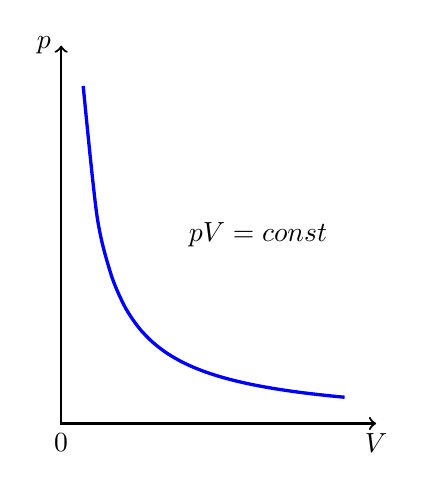
\begin{tikzpicture}[yscale=1.2]
		\draw [thick, <->] (0,4) node[left]{$p$} -- (0,0) node[below]{$0$} -- (4,0) node[below]{$V$};
		\draw [very thick,blue,domain=0.28:3.6,samples=20,smooth,variable=\x] plot (\x,{1/\x)});
		\draw (2.5,2) node{$pV=\text{const}$};
		\end{tikzpicture}
  \caption{A $p$-$V$ relation for an isothermal process is shown.}
\end{marginfigure}

If temperature $T$ remains constant, then

{

\centering

$\tcbhighmath{pV=\text{const}}$, or $\tcbhighmath{p \propto \frac{1}{V}}$

} 

In other words, the pressure $p$ of a gas is inversely proportional to volume $V$ for a gas with fixed temperature: $p_1 V_1 = p_2 V_2$

A thermodynamic process for which temperature is kept constant is called an \emph{isothermal} process.


\subsection*{Charles's law}\index{Charles's law}

Charles's law was discovered by \emph{Jacques Charles} in 1787, based on experimental observations. Of the early laws it's a favourite, because of the huge concequences:

\begin{figure*}[ht]
	\centering
	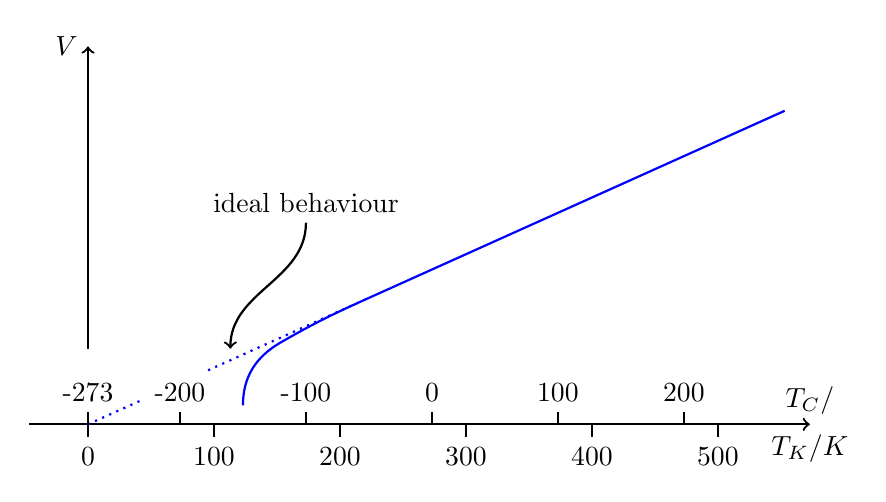
\begin{tikzpicture}[scale=1.6]
		\draw [thick, ->] (-2.73,0.6) -- (-2.73,3) node[left]{$V$};
		\draw [thick, ->] (-3.2,0) -- (3,0) node[below]{$T_K/\text{K}$} node[above]{$T_C/\OC$};
		\draw [thick,blue,domain=-0.5:2.8,samples=2,smooth,variable=\x] plot (\x,{0.45*(\x+2.73)});
		\draw [thick,blue,dotted,domain=-2.73:-0.5,samples=2,smooth,variable=\x] plot (\x,{0.45*(\x+2.73)});
		\draw [thick,blue] (-0.5,1.0035) to [out=204.2,in=30] (-1.2,0.65) to [out=210,in=90] (-1.5,0.15);
		\draw[white,fill] (-2.3,0.2) rectangle (-1.8,0.5);
		\foreach \s in {-200,-100,...,200}
		\draw [thick] (\s/100,0) --(\s/100,0.1) node[above]{\s};
		\foreach \s in {0,100,...,500}
		\draw [thick] (\s/100-2.73,0) -- (\s/100-2.73,-0.1) node[below]{\s};
		\draw [thick] (-2.73,0) -- (-2.73,0.1) node[above]{-273};
		\draw [<-, thick] (-1.6,0.6) to [out=90, in=270] (-1,1.6) node[above]{ideal behaviour};
	\end{tikzpicture}
 \caption{Charles's Law - our first glimpse of Absolute zero.}
\end{figure*}

For a fixed pressure $p$, then: $\tcbhighmath{\frac{V}{T}=\text{const}}$, or $\tcbhighmath{V \propto T}$

In other words, the volume $V$ of gas is directly proportional to its temperature $T$. 

\cmt Note that proportionality relation only applies if Kelvin scale is used

A thermodynamic process for which pressure is kept constant is called an \emph{isobaric} process

% $V$-$T$ relation for an isobaric process is shown

\cmt Charles's law implies that volume of gas tends to zero at a certain temperature, this is how the idea of \emph{absolute zero} first arose. In reality of course as $T\to0$, a real gas condenses into solid and there will be deviation from ideal behaviour (dotted line).



\subsection*{Gay-Lussac's law}\index{Gay-Lussac's law}

\begin{figure*}
	\begin{tikzpicture}
		\draw[->](0,0) -- (10,0) node[anchor=north] {$T$C};
		\draw[->](8,-0.2) -- (8,5) node[anchor=west] {$P$};
		\draw[thick, red, dashed] (1,0) -- (8,3.0975);
		\draw[thick, red] (8,3.0975) -- (9.7,3.85);
		\draw (8.1,3.175) node[color=blue] {x};
		\draw (8.4,3.25) node[color=blue] {x};
		\draw (8.7,3.4) node[color=blue] {x};
		\draw (9.0,3.5) node[color=blue] {x};
		\draw (9.3,3.65) node[color=blue] {x};
		\draw (9.6,3.75) node[color=blue] {x};
		\draw[->] (1,-1) node[anchor=north]{Absolute Zero} -- (1,-0.2);
		\end{tikzpicture}
		\caption{Pressure against Temperature of a Gas}
\end{figure*}

Gay-Lussac's law was discovered by \emph{Joseph Louis Gay-Lussac} between 1800 and 1802. If volume $V$ remains constant, then

{
	
	\centering
	
	$\tcbhighmath{\frac{p}{T}=\text{const}}$, or $\tcbhighmath{p \propto T}$
	
} 

i.e., pressure $p$ is directly proportional to temperature $T$

\cmt \piste A thermodynamic process for which volume is kept constant is called an \emph{isochoric} process, or \emph{isometric} process

The $p$-$T$ relation for an isochoric process is shown and whilst it also predicts Absolute Zero we would again expect the real behaviour to  deviate from ideal behaviour (dotted line) as $T\to0$

\section{Avogadro's Law}

This is the law commonly overlooked in textbooks - or at least, not overtly stated. 
\begin{ilight}
    Avogadro's law states that ``equal volumes of all gases, at the same temperature and pressure, have the same number of molecules.''
\end{ilight}
For a given mass of an ideal gas, the volume and amount (moles) of the gas are directly proportional if the temperature and pressure are constant.
$$\frac{V}{n}=k$$
Where
$V=$ Volume of the gas
$n=$ Amount of substance (usually in moles)
$k=$ Constant. If $n$ is in moles, this is the molar gas constant.

\subsection{An ideal gas}

With the above realationships we can build a universal pressure-temperature-volume-stuff equation sufficient to model the behaviour of real gasses. The assumptions of an ideal gas however are: 
\begin{itemize}
    \item An ideal gas is made up of numerous identical point-like molecules, spread really far apart so that the intermolecular forces are negligible;
\item Ideal gas molecules undergo random motion and obey Newton's laws of motion;
\item Ideal gas molecules undergo elastic collisions with the walls of the container the gas is in;
\item Ideal gas molecules experience only completely elastic collisions with one another.

\end{itemize}
\subsection{The ideal gas equation}

The ideal gas law was first stated by \emph{\'Emile Clapeyron} in 1834:

for a fixed amount of gas, $\tcbhighmath{\frac{PV}{T} = \text{const}}$

His work was based on the empirical Boyle's law, Charles's law, Avogadro's Law and Gay-Lussac's law

\begin{ilight}
	A gas that satisfies the equation $\tcbhighmath{pV=nRT}$ or $\tcbhighmath{pV=NkT}$ at any pressure $p$, any volume $V$, and thermodynamic temperature $T$ is called an \keypoint{ideal gas}\index{ideal gas}.
\end{ilight}

\keypoint{Molar gas constant}: $R=8.31 \text{ J mol}^{-1}\text{ K}^{-1}$

\keypoint{Boltzmann constant}: $k=1.38\times10^{-23} \text{ J K}^{-1}$

The Values of $R$ and $k$ apply for any ideal gas, i.e., they are \emph{universal} constants.

Recall conversion between number of molecules and amount of substance: $$\tcbhighmath{N=nN_A}$$

so we have a relation between the constants: $R = kN_A$, or $k=\frac{R}{N_A}$

Note that one should use \emph{thermodynamic temperature} in the equations. We can often get away with centigrade or celcius as we're usually talking about a \emph{change in temperature} and the steps are about the same size.

Thermodynamic temperature is measured in kelvins (K), so it is also called the \emph{Kelvin scale}\footnote{We will discuss in details about Kelvin scale in \S\ref{s-temp-scale} and \S\ref{s-abs-zero}.}

To convert between Kelvin temperature and Celsius temperature: $\tcbhighmath{T_K (\text{K}) \text{ } \autorightleftharpoons{\footnotesize -273}{\footnotesize +273} \text{ } T_C (\OC)}$

\subsection*{Real gases}

We always treat gasses as ideal, and indeed, real gasses behave ideally at sufficiently high temperature and low pressure.

\begin{compactitem}
	\item[--] at very low temperatures, a real gas will condense into liquid or solid.
	
	\item[--] at very high pressures, intermolecular forces become important.
\end{compactitem}

however, under normal conditions (room temperature $T \approx 300 \text{ K}$ and standard atmospheric pressure $p \approx 1.0\times10^5 \text{ Pa}$), there is no significant difference between a real gas and an ideal gas so the ideal gas approximation can be used with good accuracy for most of our applications.

\example{A sealed cylinder of volume of 0.050 m$^3$ contains 75 g of air. The molar mass of air is 29 g mol$^{-1}$. (a) Find the air pressure when its temperature is $30^\circ$C. (b) The gas is allowed to expand with its pressure fixed. Find the temperature of the gas when the volume doubles.}

\begin{soln}
    
amount of gas: $n=\frac{m}{M} = \frac{75}{29} \approx 2.59 \text{ mol}$

pressure at $30^\circ$C: $p = \frac{nRT_1}{V_1} = \frac{2.59\times8.31\times(30+273)}{0.050} \approx 1.30\times10^5 \text{ Pa}$


pressure fixed, so $V \propto T \RA \frac{T_2}{T_1} = \frac{V_2}{V_1} = 2 \RA T_2 = 2\times (30+273) = 606 \text{ K} = 333^\circ\text{C}$ \end{soln}

\example{A gas cylinder holding 5000 cm$^3$ of air at a temperature of 27 $^\circ$C and a pressure of $6.0\times10^5 \text{ Pa}$ is used to fill balloons. Each balloon contains 1000 cm$^3$ of air at 27 $^\circ$C and $1.0\times10^5$ Pa when filled. (a) Find the initial amount of gas in the cylinder. (b) Find the number of balloons that can be filled.}

\begin{soln} initial amount of gas in cylinder: $n_0 = \frac{p_0 V}{RT} = \frac{9.0\times10^5\times5000\times10^{-6}}{8.31\times(27+273)} \approx 1.203 \text{ mol}$

final amount of gas in cylinder: $n_\text{remain} = \frac{pV}{RT} = \frac{1.0\times10^5\times5000\times10^{-6}}{8.31\times(27+273)} \approx 0.201 \text{ mol}$

Air will leave the cylinder to fill balloons only if pressure inside the cylinder is higher than pressure of the balloon. When the two pressures become equal, no more balloons can be filled, there will be some air remain in cylinder...

amount of gas in each balloon: $n_\text{b} = \frac{pV_b}{RT} = \frac{1.0\times10^5\times1000\times10^{-6}}{8.31\times(27+273)} \approx 0.040 \text{ mol}$

number of balloons: $N = \frac{n_0 - n_\text{remain}}{n_\text{b}} = \frac{1.203-0.201}{0.040} \approx 25$ \end{soln}

\example{A storage cylinder has a volume of $5.0\times10^{-4}\text{ m}^3$. The gas is at a temperature
	of 300 K and a pressure of $4.0 \times 10^6$ Pa.	(a) Find the number of molecules in the cylinder. (b) The gas molecules slowly leak from the cylinder at a rate of $1.6 \times 10^{16} \text{ s}^{-1}$. Find the time, in days, after which the pressure will reduce by 5.0\%.}

\begin{soln} initial number of molecules: $N_0 = \frac{p_0V}{kT} = \frac{4.0\times10^6\times 5.0\times10^{-4}}{1.38\times10^{-23}\times300}\approx 4.83\times10^{23}$

\eqyskip

volume fixed, so $N \propto p \RA \frac{\Delta N}{N_0} = \frac{\Delta p}{p_0} = 5.0\%$

number of molecules escaped: $\Delta N = 0.05\times4.83\times10^{23} \approx 2.42 \times10^{22}$

time needed: $t = \frac{2.42 \times10^{22}}{1.6 \times 10^{16}} \approx 1.51 \times 10^6 \text{ s} \approx 17.4 \text{ days}$ \end{soln}

\newpage %%%%

\question{Containers $A$ has a volume of $2.5\times10^{-2} \text{ m}^3$ contains a gas at a temperature of 17$^\circ$C and pressure of $1.3 \times 10^5 \text{ Pa}$ and . Another container $B$ of same size holds a gas at same temperature and a pressure of $1.9 \times 10^5 \text{ Pa}$. The two containers are initially isolated from each another. (a) Find the total amount of molecules. (b) The two containers are now connected through a tube of negligible volume. Assume the temperature stays unchanged, find the final pressure of the gas.}

\question{The air in a car tyre can be assumed to have a constant volume of $3.0\times10^{-2} \text{ m}^3$}. The pressure of this air is $2.8\times10^5 \text{ Pa}$ at a temperature of $25^\circ$C. The pressure is to be increased using a pump. On each stroke 0.015 mol of air is forced into the tyre. If gas has a final pressure of $3.6\times10^5 \text{ Pa}$ and final temperature of $28^\circ$C. Find the number of strokes of the pump required.



\subsection{The kinetic theory of ideal gases}

\keypoint{Kinetic model of gases}\index{kinetic model of gases}: a theory based on microscopic motion of molecules of a gas that explains its macroscopic properties

\subsection{Assumptions of ideal gas model}


\begin{ilight}
	
kinetic theory of the ideal gas model is based on the following assumptions:

\begin{compactitem}
	
\item[--] gas molecules are in constant \emph{random} motion
	
\item[--] \emph{intermolecular separation} is much greater than size of molecules

volume of molecules is negligible compared to volume occupied by gas

\item[--] \emph{intermolecular forces} are negligible

\item[--] collisions between molecules are perfectly \emph{elastic}, i.e., no kinetic energy lost

\item[--] molecules travel in straight line between collisions
\end{compactitem}

\end{ilight}

\example{A mass of 20 g helium-4 at a temperature of 37$^\circ$C has a pressure of $1.2\times10^5 \text{ Pa}$. Each helium-4 atom has a diameter of 280 pm. (a) Find the volume occupied by the gas and the volume of atoms in this gas. (b) Compare the two volumes, suggest whether this gas can be considered as an ideal gas.}

\begin{soln}
    
number of helium molecules: $N = nN_A = \frac{m}{M} \times N_A = \frac{20}{4.0} \times 6.02\times10^{23} \approx 3.01\times10^{24} $

\eqyskip

volume of gas: $V_\text{gas} = \frac{NkT}{p} = \frac{3.01\times10^{24}\times1.38\times10^{-23}\times (37+273)}{1.2\times10^5} \approx 0.107 \text{ m}^3$

\eqyskip

volume of one atom: $V_\text{atom} = \frac{4}{3}\pi r^3 = \frac{4}{3} \pi\times(140\times10^{-12})^3 \approx 1.15\times10^{-29} \text{ m}^3$

volume of all atoms: $V_\text{atoms} = N V_\text{atom} = 3.01\times10^{24} \times 1.15\times10^{-29} \text{ m}^3 \approx 3.46 \times 10^{-5} \text{ m}^{3}$

$V_\text{gas} \gg V_\text{atoms}$, so this gas can approximate to an ideal gas \end{soln}


\subsection{Pressure (quantitative view)}

The pressure of gas on a container is due to collision of gas molecules with container. To derive an expression for this, let's first consider the effect of one single molecule moving in one dimension only, and then generalise the result to a gas containing $N$ molecules moving in all three dimensions.

\begin{figure}[ht]
\centering
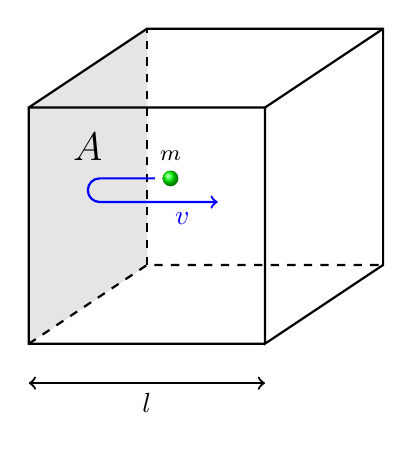
\begin{tikzpicture}[scale=1]
\coordinate (A) at (0,0); 
\coordinate (B) at (3,0);
\coordinate (C) at (4.5,1); 
\coordinate (D) at (1.5,1);
\coordinate (E) at (0,3); 
\coordinate (F) at (3,3);
\coordinate (G) at (4.5,4); 
\coordinate (H) at (1.5,4);
\draw [gray!20,fill] (A) -- (D) -- (H) -- (E) -- cycle;
\draw [thick] (B) -- (A) -- (E) -- (F) -- (B) -- (C) -- (G) -- (H) -- (E);
\draw [thick] (F) -- (G);
\draw [thick,dashed] (A) -- (D) -- (C);
\draw [thick,dashed] (D) -- (H);
\draw [thick,blue,->] (1.6,2.1) -- (0.9,2.1) to [out=180,in=90] (0.75,1.95)to [out=-90,in=180] (0.9,1.8) -- (2.4,1.8) node[below, pos=0.7]{$v$};
\shade [ball color = green] (1.8,2.1) circle [radius=0.1];
\draw [thick,<->] (0,-0.5) -- (1.5,-0.5) node[below]{$l$} -- (3,-0.5);
\node at (0.75,2.5) {{\Large $A$}};
\node[above] at (1.8,2.2) {{\footnotesize $m$}};
\end{tikzpicture}

\caption{One gas molecule moving in 1-D}
\label{onedmol}
\end{figure}

Let's assume this single molecule only moves in $x$-direction (see figure \ref{onedmol}). The change in momentum when colliding with wall: $\Delta P_x = mv_x - (-mv_x) = 2mv_x$\footnote{In this chapter we use $P$ for momentum of a particle and $p$ for pressure of a gas to avoid confusion.}

The time interval between collisions: $\Delta t=\frac{2l}{v_x}$

So the average force: $F_x=\frac{\Delta P_x}{\Delta t} = \frac{2mv_x}{\tfrac{2l}{v_x}} = \frac{mv_x^2}{l}$

aWhich in turn leads to the average pressure: $p_x=\frac{F}{A} = \frac{mv_x^2}{lA} = \RA p_x = \frac{mv_x^2}{V}$

We finally need to generalise to $N$ molecules moving in 3-D;

\begin{compactitem}
	\item[--] $N$ molecules so $N$ times the contributions to pressure
	
	but there is a \emph{distribution} of speeds for $N$ molecules, so should take average of $v^2$
	
	\item[--] in three-dimensional space, we have: $v^2=v_x^2 + v_y^2 + v_z^2$
	
	but molecules have no preference in any specific direction, so: $\avg{v_x^2} = \avg{v_y^2} = \avg{v_z^2} = \frac{\avg{v^2}}{3}$
	
	pressure should be shared equally among three dimensions: $p=p_x=p_y=p_z$
		
\end{compactitem}


therefore we find the pressure of an ideal gas is given by: $$\tcbhighmath{p = \frac{Nm\avg{v^2}}{3V}}$$

\cmt Where $\avg{v^2}$ is the \emph{mean square velocity} of gas molecules.

we can further define r.m.s. (root mean square) velocity: $v_\text{rms} = \sqrt{\avg{v^2}}$ .

Note that the gas molecules in random motion so there exists a range of velocities. We have to treat the molecules statistically - in other words, we cannot tell exact velocity of a specific molecule, but can only tell mean values.

\cmt If $N$ is number of molecules, and $m$ is mass of one molecule then $Nm$ gives total mass of the gas, and $\frac{Nm}{V}$ gives gas density $\rho$

we can rewrite the pressure formula as: $$\tcbhighmath{p=\frac{1}{3}\rho \avg{v^2}}$$ 

This shows clearly that pressure depends only on density and mean square speed of molecules and leads to some useful conclusions:
\begin{compactitem}
\item[--] $N \up$ $\ra$ more molecules, more collisions $\ra p\up$

\item[--] $m \up$ $\ra$ greater mass, greater force upon collision $\ra p\up$

\item[--] $v \up$ $\ra$ strike container harder, also more often $\ra p\up$

\item[--] $V \up$ $\ra$ spend more time in gas, less frequent collision with container $\ra p\down$
\end{compactitem}


\subsection{Kinetic energy of a gas}

We have assembled two equations for ideal gases:
\begin{equation*}
\left\{
	\begin{array}{ll}
	pV = nRT \, \text{, or } \, pV = NkT &\quad \text{ideal gas law} \\
	p = \frac{Nm\avg{v^2}}{3V} &\quad \text{pressure law}
	\end{array} \right.
\end{equation*}

If we compare the two equations: $$pV=\frac{1}{3}Nm\avg{v^2}=NkT \RA m\avg{v^2}=3kT$$

It becomes clear that we have an expression for the \emph{mean kinetic energy} of a single molecule in a gas: $$\tcbhighmath{\avg{E_k}=\frac{1}{2}m\avg{v^2}=\frac{3}{2}kT}$$

This mean K.E. of ideal gas molecules is \emph{proportional} to its thermodynamic temperature - it can be helpful to think about the link with molecular speeds: $\tcbhighmath{v_\text{rms}^2 \propto T}$

Recall that a higher temperature means higher speed for molecules but we only talk about \emph{translational} K.E. here - molecules have this energy because they are moving through space. The total kinetic energy may also include \emph{rotational} K.E. and \emph{vibrational} K.E.
\footnote{There is an important result in classical thermal physics, known as the \emph{equipartition of energy theorem}. It states that the average energy per molecule is $\frac{1}{2}kT$ for each independent \emph{degree of freedom}. A molecule can move in three directions, corresponding to three translational degrees of freedom, thus its mean translational kinetic energy is $\frac{3}{2}kT$. For a polyatomic gas (each molecule consists of several atoms), apart from translational motion , it has additional rotational degrees of freedom and different vibrational modes, so its average energy can be calculated by counting the total number of degrees of freedom.}

$$\avg{E_k} = \frac{3}{2}k T$$ gives the \emph{mean}, or \emph{average} K.E. per molecule. The gas molecules exchange energies with each other upon collisions so for any individual molecule, the K.E. is not a constant. The mean K.E. however is constant, which depends on temperature $T$ only. In a mixture of several gases, K.E. is shared \emph{equally} among its components because of repeated collisions between particles. What this means in practive is that all molecules have same K.E., so heavier molecules will move more slowly.

\example{Air consists of oxygen (O$_2$, molar mass $32\text{ g mol}^{-1}$) and nitrogen (N$_2$, molar mass $28\text{ g mol}^{-1}$). (a) Calculate the mean translational kinetic energy of these molecules at 300 K. (b) Estimate the typical speed for each type of the molecule.}

\begin{soln} mean K.E. of single molecule: $\avg{E_k} = \frac{3}{2}kT = \frac{3}{2} \times 1.38\times10^{-23} \times 300 \approx 6.21\times 10^{-21} \text{ J}$

{
	
	\centering
	
	$\avg{E_k} = \frac{1}{2}m\avg{v^2} = \frac{3}{2} kT \RA \frac{1}{2} \frac{M}{N_A} \avg{v^2} = \frac{3}{2} kT \RA \avg{v^2} = \frac{3kN_AT}{M} = \frac{3RT}{M}$
	
}

\eqyskip

for oxygen molecule: $v_\text{O$_2$} \approx  \sqrt{\frac{3\times8.31\times300}{0.032}} \approx 483 \mps$

\eqyskip

for nitrogen molecule: $v_\text{N$_2$} \approx  \sqrt{\frac{3\times8.31\times300}{0.028}} \approx 517 \mps$ \end{soln}

\example{A cylinder container initially holds a gas of helium-4 at a temperature of 54\OC. (a) Find the mean square speed of these helium atoms. (b) If the temperature is raised to 540\OC, find the r.m.s. speed of the atoms.}

\begin{soln} mass of one helium-4 atom: $m=4\text{u} = 4\times 1.66\times10^{-27} \approx 6.64\times10^{-27} \text{ kg}$

at 54\OC: $\, \frac{1}{2}m\avg{v^2} = \frac{3}{2}kT \RA \avg{v^2} = \frac{3kT}{m} = \frac{3\times1.38\times10^{-23}\times(54+273)}{6.64\times10^{-27}} \approx 2.04 \times 10^6 \text{ m}^2 \text{ s}^{-2}$

\eqyskip 

note relation between $v$ and $T$: $\, \avg{v^2} \propto T \RA \frac{\avg{v^{\prime 2}}}{\avg{v^2}} = \frac{T'}{T} \RA v'_\text{rms} = \sqrt{\frac{T'}{T}}\times v_\text{rms}$

\eqyskip 

at 540\OC: $\, v'_\text{rms} = \sqrt{\frac{540+273}{54+273}} \times \sqrt{2.04 \times 10^6} \approx 2.25 \times 10^3 \mps$ \end{soln}


\question{A fixed mass of gas expands to twice its volume at constant temperature. (a) How does its pressure change? (b) How does mean kinetic energy change?}

\question{In order for a molecule to escape from the gravitational field of the earth, it must have a speed of $1.1\times10^6\mps$ at the top of the atmosphere. (a) Estimate the temperature at which helium-4 atoms could have this speed. (b) Helium atom actually escape from top of the atmosphere at much lower temperatures, explain how this is possible.}